\documentclass{article}
\usepackage{tikz}
\usetikzlibrary{arrows.meta,positioning,calc,shapes.geometric}
\pagestyle{empty}
\begin{document}
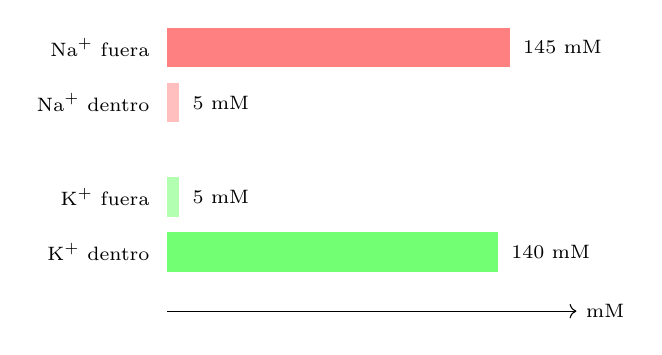
\begin{tikzpicture}

\def\bar#1#2#3#4{\fill[#4] (2.2,#1) rectangle ({2.2+#2*0.03},{#1+0.5}); \node[left, font=\scriptsize] at (2.1,{#1+0.25}) {#3}; \node[right, font=\scriptsize] at ({2.25+#2*0.03},{#1+0.25}) {#2 mM};}
\bar{3.6}{145}{Na$^+$ fuera}{red!50}
\bar{2.9}{5}{Na$^+$ dentro}{red!25}
\bar{1.7}{5}{K$^+$ fuera}{green!30}
\bar{1.0}{140}{K$^+$ dentro}{green!55}
\draw[->] (2.2,0.5) -- (7.4,0.5) node[right, font=\scriptsize] {mM};

\end{tikzpicture}
\end{document}
